\section{Overview of the SRAM Structure}
\label{sec:overview}


% address decode and mem array
The baseline SRAMs generated by OpenRAM have 1 read/write port as
shown in Figure~\ref{fig:sram_architecture}. The address is decoded
(Section~\ref{sec:addressdecoder}) into a one-hot set of word lines
(WL) which are driven by word line drivers
(Section~\ref{sec:wldriver}) over the bit-cell array
(Section~\ref{sec:bitcellarray}). To facilitate reads, the precharge
circuitry (Section~\ref{sec:precharge}) precharges the bitlines so
that the column mux (Section~\ref{sec:column_mux}) can select the
appropriate word which is then sensed by the sense amplifiers
(Section~\ref{sec:senseamp}).  Write drivers
(Section~\ref{sec:writedriver}) use the bidirectional nature of the
column mux to write the appropriate columns in a given memory row.

A representative layout of such a memory closely resembles the logical
representation and is shown in Figure~\ref{fig:layout_view}.  The
address and data flip-flops and control circuitry are not shown but
are detailed in Section~\ref{sec:control}.


\begin{figure}[htb]
\centering
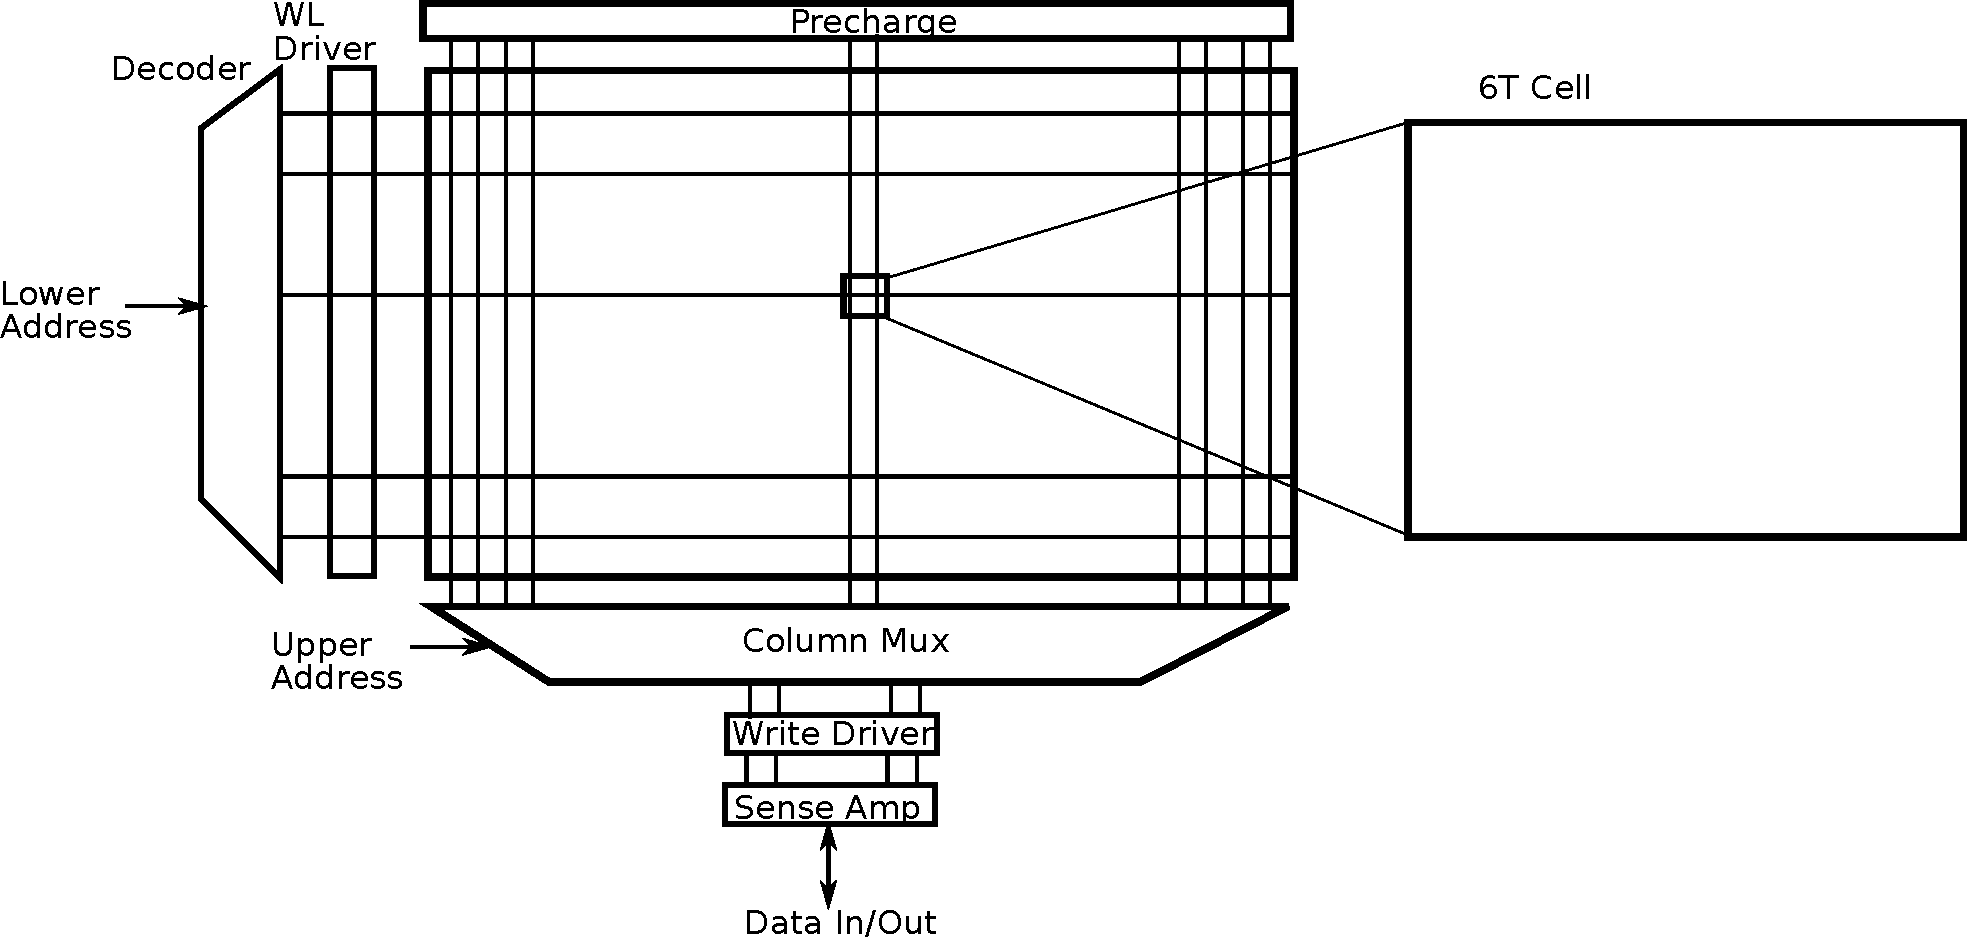
\includegraphics[width=10cm]{./figs/sram_overview.pdf}
\caption{Single Port SRAM Architecture}
\label{fig:sram_architecture}
\end{figure}


\begin{figure}[htb]
\centering
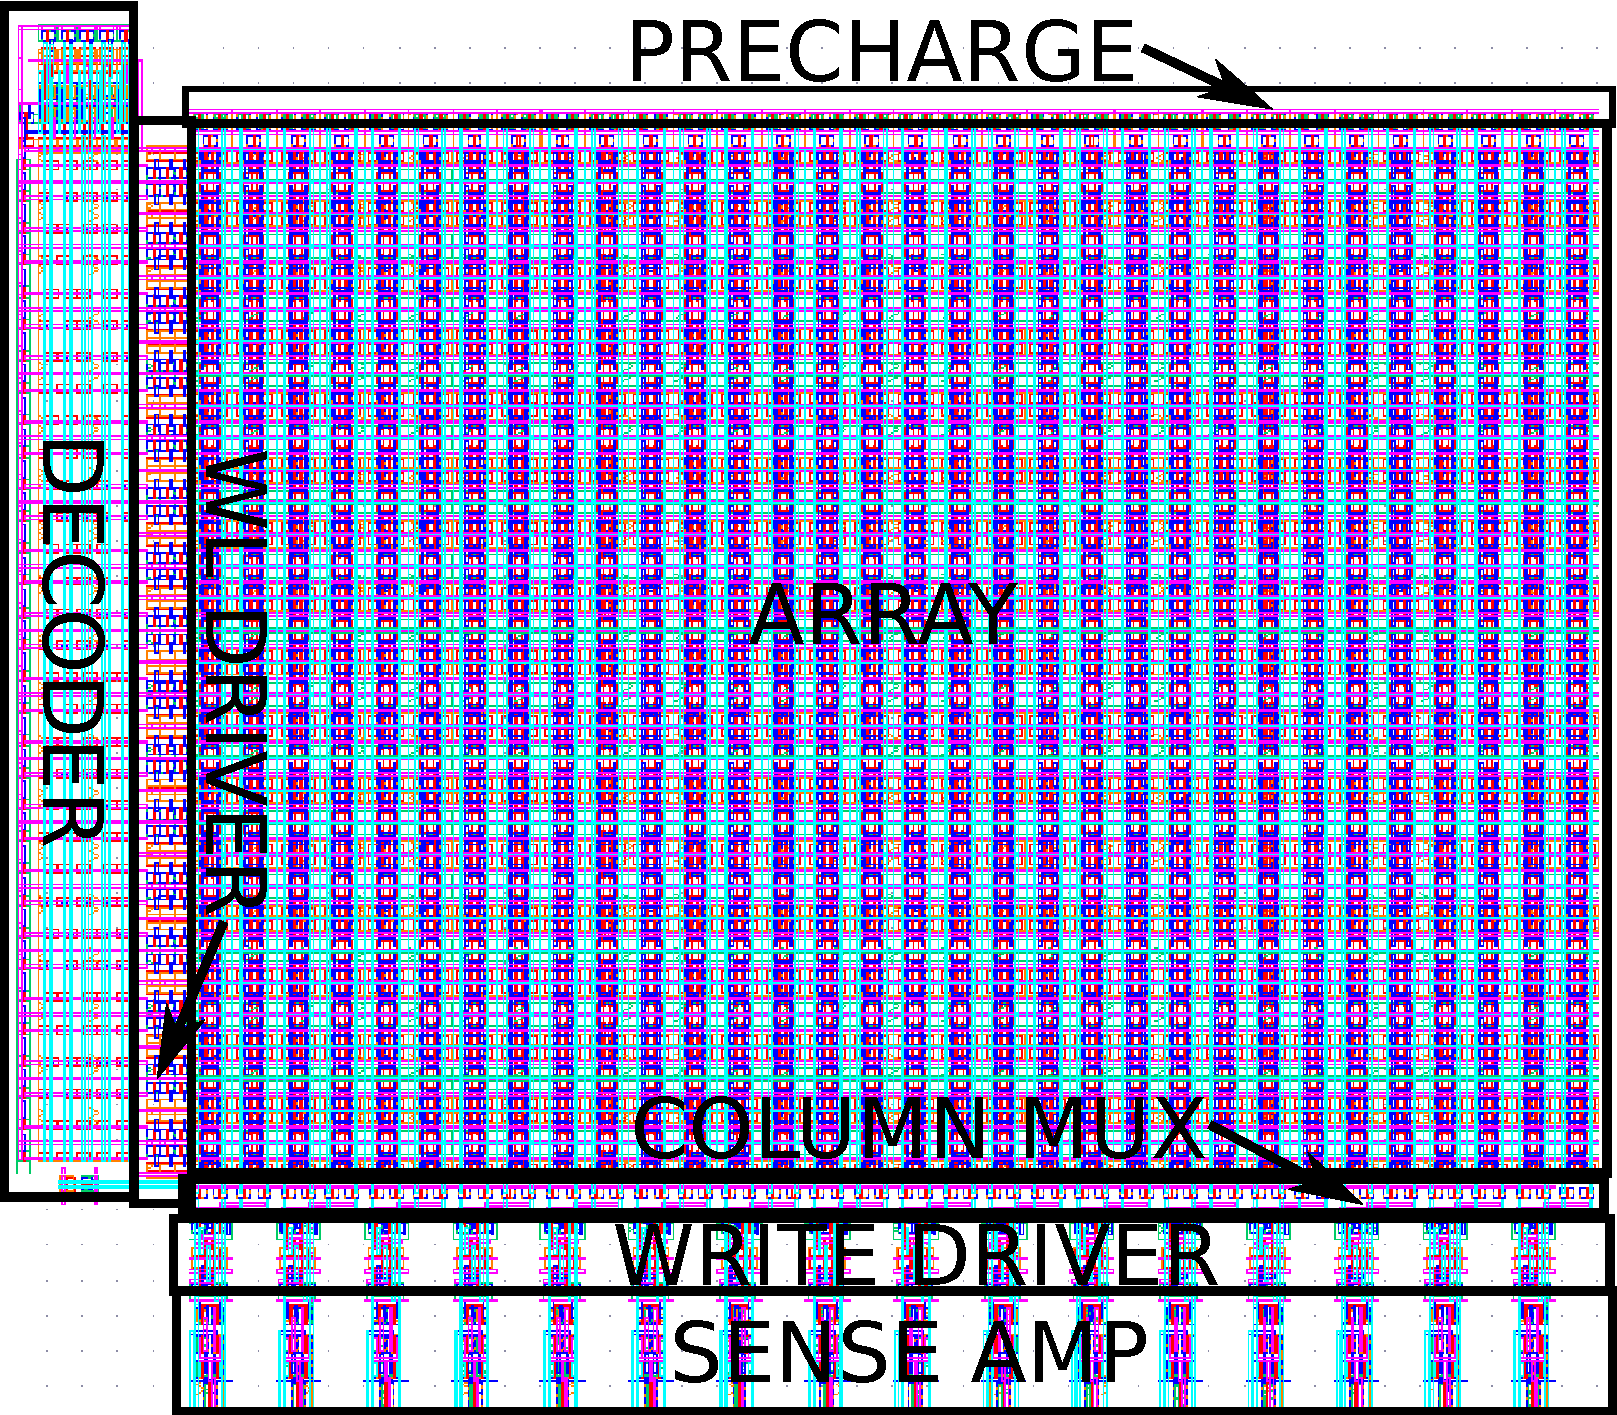
\includegraphics[width=6cm]{./figs/layout_view_1024_16_annotated.pdf}
\caption{1k SRAM with Two Columns and 16-bit Data}
\label{fig:layout_view}
\end{figure}



\subsection{Inputs/Outputs}
\label{sec:io}

The inputs to the SRAM are: 
\begin{itemize}
\setlength{\itemsep}{0pt}
\item clk - External Clock
\item CSb - Active-low Chip Select
\item WEb - Active-low Write Enable
\item OEb - Active-low Output Enable
\item ADDR[\#] - Address Bus input (LSB is 0)
\item DATA[\#] - Bi-directional Data bus (LBS is 0)
\end{itemize}
If multiple ports are used, the ADDR and DATA buses are appended with
integers to extend them.

The outputs to the SRAM are: 
\begin{itemize}
\setlength{\itemsep}{0pt}
\item DATA\# - correspond to the bi-directional Data bus.
\end{itemize}

The supply voltages to the SRAM are:
\begin{itemize}
\item vdd - Supply voltage
\item gnd - Ground supply voltage
\end{itemize}

\subsection{Top-Level SRAM Module}
\label{sec:sram}

The sram class in \verb|sram.py| is the top-level SRAM module.  This
class handles the overall organization of the memory, instantiates the
contorl logic, instantiates a number of banks, and creates decoded
enable signals for multiple banks. All of the top level routing is
performed in the sram class.


The sram class instantiates identical copies of the bank module from
\verb|bank.py|.  All other sub-modules access the value of sizes from
bank.  The bank module includes an address decoder, (optional) column
address decoder, (optional) column mux, sense amplifiers, precharge
circuitry, write drivers, etc.  A single bank organization is depicted
in Figure~\ref{fig:sram_architecture}.

Discussion of the design data structure is discussed in
Section~\ref{sec:design} and the modules contained in the top-level
SRAM are detailed in Section~\ref{sec:modules}.

